\documentclass{standalone}
\usepackage{tikz}
\usetikzlibrary{arrows.meta, positioning, backgrounds}

\begin{document}

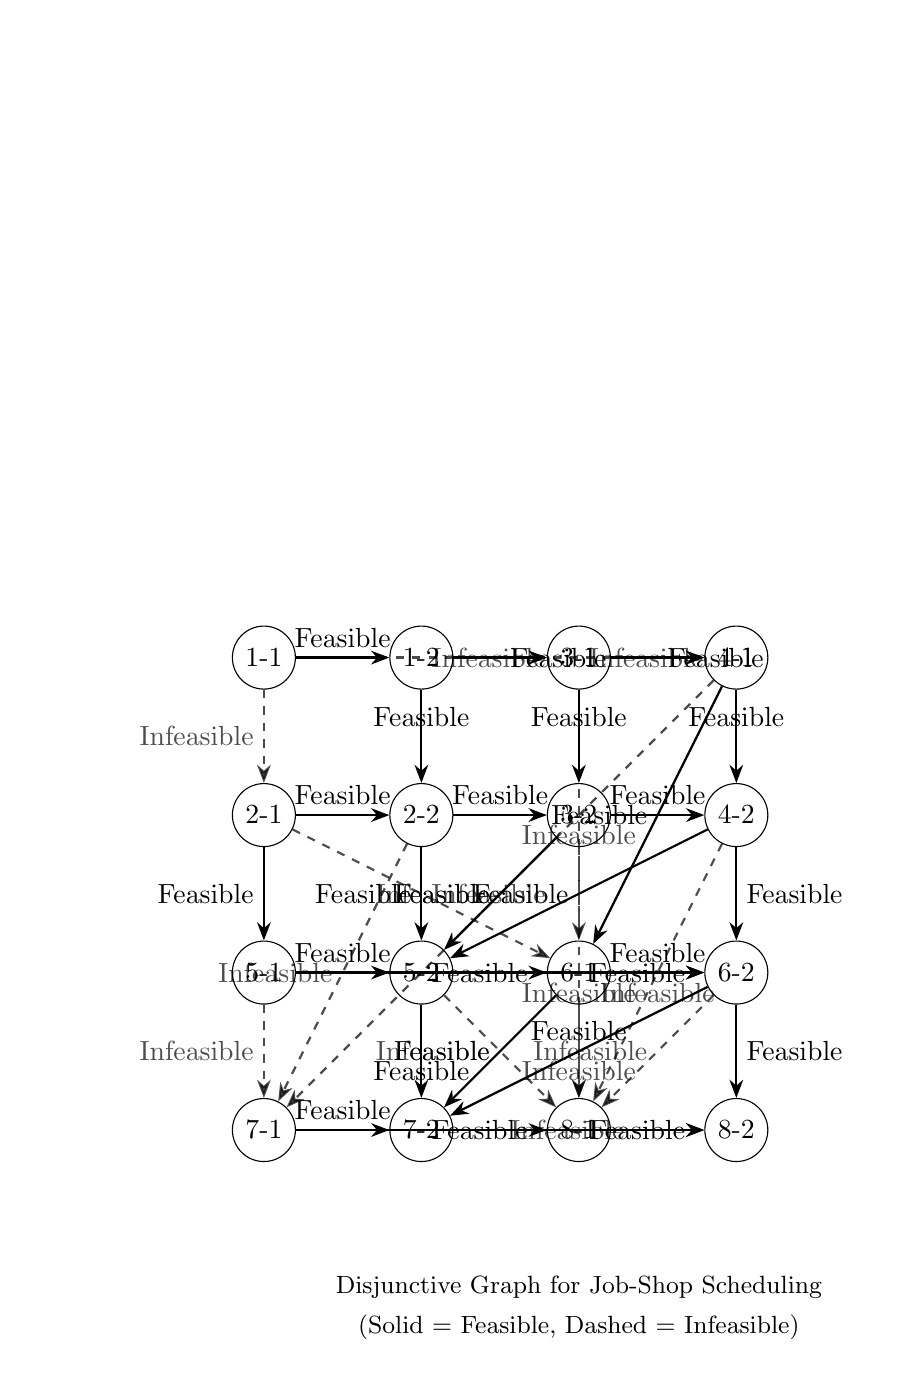
\begin{tikzpicture}[
  node distance=10mm and 10mm,
  operation/.style={circle, draw, minimum size=8mm, inner sep=0pt},
  feasible/.style={-Stealth, thick},
  infeasible/.style={dashed, -Stealth, thick, opacity=0.7}
]

% Background rectangle (white)
\fill[white] (-3,-3) rectangle (8,8);

% Define nodes
\node[operation] (op11) at (0,0) {1-1};
\node[operation] (op12) at (2,0) {1-2};
\node[operation] (op21) at (0,-2) {2-1};
\node[operation] (op22) at (2,-2) {2-2};
\node[operation] (op31) at (4,0) {3-1};
\node[operation] (op32) at (4,-2) {3-2};
\node[operation] (op41) at (6,0) {4-1};
\node[operation] (op42) at (6,-2) {4-2};
\node[operation] (op51) at (0,-4) {5-1};
\node[operation] (op52) at (2,-4) {5-2};
\node[operation] (op61) at (4,-4) {6-1};
\node[operation] (op62) at (6,-4) {6-2};
\node[operation] (op71) at (0,-6) {7-1};
\node[operation] (op72) at (2,-6) {7-2};
\node[operation] (op81) at (4,-6) {8-1};
\node[operation] (op82) at (6,-6) {8-2};

% Draw edges (disjunctive)
% From op11 to next operations
\draw[feasible] (op11) -- (op12) node[midway, above] {Feasible};
\draw[infeasible] (op11) -- (op21) node[midway, left] {Infeasible};
\draw[infeasible] (op11) -- (op31) node[midway, right] {Infeasible};

% From op12 to next
\draw[feasible] (op12) -- (op22) node[midway, above] {Feasible};
\draw[feasible] (op12) -- (op31) node[midway, right] {Feasible};
\draw[infeasible] (op12) -- (op41) node[midway, right] {Infeasible};

% From op21 to next
\draw[feasible] (op21) -- (op22) node[midway, above] {Feasible};
\draw[feasible] (op21) -- (op51) node[midway, left] {Feasible};
\draw[infeasible] (op21) -- (op61) node[midway, right] {Infeasible};

% From op22 to next
\draw[feasible] (op22) -- (op32) node[midway, above] {Feasible};
\draw[feasible] (op22) -- (op52) node[midway, left] {Feasible};
\draw[infeasible] (op22) -- (op71) node[midway, left] {Infeasible};

% From op31 to next
\draw[feasible] (op31) -- (op32) node[midway, above] {Feasible};
\draw[feasible] (op31) -- (op41) node[midway, right] {Feasible};
\draw[infeasible] (op31) -- (op61) node[midway, below] {Infeasible};

% From op32 to next
\draw[feasible] (op32) -- (op42) node[midway, above] {Feasible};
\draw[feasible] (op32) -- (op52) node[midway, left] {Feasible};
\draw[infeasible] (op32) -- (op81) node[midway, below] {Infeasible};

% From op41 to next
\draw[feasible] (op41) -- (op42) node[midway, above] {Feasible};
\draw[feasible] (op41) -- (op61) node[midway, left] {Feasible};
\draw[infeasible] (op41) -- (op71) node[midway, left] {Infeasible};

% From op42 to next
\draw[feasible] (op42) -- (op52) node[midway, left] {Feasible};
\draw[feasible] (op42) -- (op62) node[midway, right] {Feasible};
\draw[infeasible] (op42) -- (op81) node[midway, below] {Infeasible};

% From op51 to next
\draw[feasible] (op51) -- (op52) node[midway, above] {Feasible};
\draw[feasible] (op51) -- (op61) node[midway, right] {Feasible};
\draw[infeasible] (op51) -- (op71) node[midway, left] {Infeasible};

% From op52 to next
\draw[feasible] (op52) -- (op62) node[midway, right] {Feasible};
\draw[feasible] (op52) -- (op72) node[midway, below] {Feasible};
\draw[infeasible] (op52) -- (op81) node[midway, left] {Infeasible};

% From op61 to next
\draw[feasible] (op61) -- (op62) node[midway, above] {Feasible};
\draw[feasible] (op61) -- (op72) node[midway, left] {Feasible};
\draw[infeasible] (op61) -- (op81) node[midway, below] {Infeasible};

% From op62 to next
\draw[feasible] (op62) -- (op72) node[midway, above] {Feasible};
\draw[feasible] (op62) -- (op82) node[midway, right] {Feasible};
\draw[infeasible] (op62) -- (op81) node[midway, left] {Infeasible};

% From op71 to next
\draw[feasible] (op71) -- (op72) node[midway, above] {Feasible};
\draw[feasible] (op71) -- (op81) node[midway, right] {Feasible};
\draw[infeasible] (op71) -- (op82) node[midway, right] {Infeasible};

% From op72 to next
\draw[feasible] (op72) -- (op82) node[midway, right] {Feasible};

% Add labels for the graph type
\node at (4,-8) {\small Disjunctive Graph for Job-Shop Scheduling};
\node at (4,-8.5) {\small (Solid = Feasible, Dashed = Infeasible)};

\end{tikzpicture}

\end{document}